\documentclass[8pt, jfont=ipaexm, t]{beamer} % IPAex明朝
\usepackage{hyperref}
% 一般的によく使用されるパッケージ
\usepackage{caption}
\usepackage[utf8]{inputenc}
\usepackage{graphicx}
\usepackage{amsmath}
\usepackage{amsfonts}
\usepackage{amssymb}
\usepackage{tikz}
\usepackage{pgfplots}
%\usepackage{xeCJK}
%\usetheme{Copenhagen}
\pgfplotsset{compat=1.17}
\usepackage{listings}
% \usepackage{slashbox}

% スタイル設定
\usepackage{ifthen}
\usepackage[varg]{txfonts}
\usepackage{ragged2e}
\usepackage{svg}
\usepackage{xcolor}
\usepackage{url}
\usepackage{bm}
\usepackage{pgfplots}
\pgfplotsset{compat=1.18}

\usetikzlibrary{graphs}
\usetikzlibrary {arrows.meta}
\usetikzlibrary {bending}
\usetikzlibrary{arrows,shapes,automata,petri,positioning,calc}


% 和文用パッケージ(luatex用)
\usepackage{luatexja}
\usepackage{luatexja-fontspec}
\usepackage{lmodern}
\usepackage[T1]{fontenc} % 必要に応じてフォントエンコーディングを指定


%カラーテーマの選択(省略可)
\usecolortheme{orchid}
%フォントテーマの選択(省略可)
\usefonttheme{professionalfonts}
%フレーム内のテーマの選択(省略可)
\useinnertheme{circles}
%フレーム外側のテーマの選択(省略可)
\useoutertheme{infolines}
%しおりの文字化け解消
% \AtBeginShipoutFirst{\special{pdf:tounicode EUC-UCS2}}

% \AtBeginShipoutFirst{\special{pdf:tounicode 90ms-RKSJ-UCS2}}
%ナビゲーションバー非表示
%\setbeamertemplate{navigation symbols}{}

% タイトル色
\setbeamercolor{title}{fg=structure, bg=}

% フレームタイトル色
\setbeamercolor{frametitle}{fg=structure, bg=}

% caption に番号追加
\setbeamertemplate{caption}[numbered]
% caption 日本語
\renewcommand{\figurename}{図}
\renewcommand{\tablename}{表}

\usepackage[export]{adjustbox} % loads also graphicx


\usetheme[progressbar=frametitle, block=fill, numbering=fraction,]{metropolis}
% \usetheme{default}
            
% ブロックのスタイルをカスタマイズ
\setbeamertemplate{blocks}[rounded]
\setbeamercolor{block title}{bg=gray!30,fg=black} % ブロックのタイトルの背景とフォントの色
\setbeamercolor{block body}{bg=gray!10,fg=black} % ブロック本体の背景とフォントの色

\setbeamercolor{block title example}{bg=orange!30,fg=black} % 例のブロックのタイトルの背景とフォントの色
\setbeamercolor{block body example}{bg=orange!10,fg=black} % 例のブロック本体の背景とフォントの色

\setbeamercolor{block title alerted}{bg=red!30,fg=black} % アラートのブロックのタイトルの背景とフォントの色
\setbeamercolor{block body alerted}{bg=red!10,fg=black} % アラートのブロック本体の背景とフォントの色

\tikzset{set label/.style={fill=white,circle,inner sep=2}}

\def\radius{2}
\def\ratio{0.6}

\def\centerA{180:\ratio*\radius}
\def\circleA{(\centerA) circle [radius=\radius]}





%追加
\setbeamertemplate{footline}{%
  \hfill%
  \usebeamercolor[fg]{page number in head/foot}%
  \usebeamerfont{page number in head/foot}%
  \insertframenumber\,/\,\inserttotalframenumber\kern1em\vskip2pt%
}

%ソースコードに関する設定
\lstset{
  basicstyle={\ttfamily},
  identifierstyle={\small},
  commentstyle={\smallitshape},
  keywordstyle={\small\bfseries},
  ndkeywordstyle={\small},
  stringstyle={\small\ttfamily},
  frame={tb},
  breaklines=true,
  columns=[l]{fullflexible},
  numbers=left,
  % xrightmargin=0zw,
  % xleftmargin=3zw,
  numberstyle={\scriptsize},
  stepnumber=1,
  numbersep=1,
  lineskip=1ex
}


\tikzset{
    place/.style={
        circle,
        thick,
        draw=black,
        fill=gray!50,
        minimum size=6mm,
    },
        state/.style={
        circle,
        thick,
        draw=blue!75,
        fill=blue!20,
        minimum size=6mm,
    },
}



\title{ディジタル画像処理}
\institute{画像情報工学研究室}
\author{佐藤謙成}
\date{\today}

\begin{document}
\maketitle

\begin{frame}{目次}
  \tableofcontents
\end{frame}

\section{表色系}

\begin{frame}{表色系}
表色系(color specification
system)とは,色を定量的に表す体系のことを指す.表色系には顕色系と混色系の2種類存在し,マンセル表色系は顕色系,CIE-RGP表色系やCIE-XYZ表色系は混色系である.
\end{frame}

\section{マンセル表色系}

\begin{frame}{マンセル表色系とは}
マンセル表色系とは,米国の画家マンセルが,色相,明度,彩度の3属性で定義した色表示方法のことである
\begin{itemize}
\item 色相とは,色の違いを示す属性である.赤,黄,緑,青,紫の5種類を基本色相としてその中間にそれぞれ10等分することで全体を100色相とする.
\item 明度とは,各色相の明るさを示す属性である.黒を0段階,白を10段階とした11段階に等分割にして表現する.
\item 彩度とは,色の鮮やかさを示す属性である.各色相と明度ごとに無彩色から最も鮮やかな色までを等間隔で区切り,数字で表現する.
\end{itemize}
\begin{figure}[h]
  \centering
  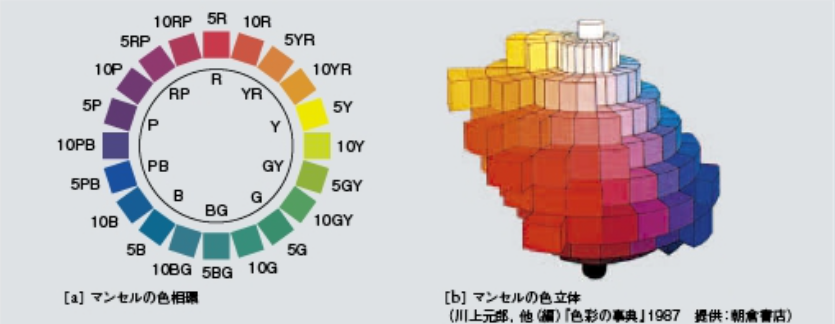
\includegraphics[width=0.5\textwidth]{./figure/021.png}
  \caption{マンセル表色系の色相環と色立体}
\end{figure}
\end{frame}

\section{CIE-RGB表色系}
\begin{frame}{CIE-RGB表色系とは}
CIE-RGB表色系とは,赤,緑,青を原色とし,それを加法することによる色表示方法のことである.
測定対象からの反射光を \(\textbf{C}\) , 原刺激を \(\textbf{R, G, B}\)
としてそれぞれの刺激値をR, G, Bとして混色したときに

\begin{equation} \label{eq:Crgb}
\textbf{C} = R\textbf{R} + G\textbf{G} + B\textbf{B}
\end{equation}

式\eqref{eq:Crgb}を満たしたときに,両者は等色であるという.

\begin{figure}[h]
  \centering
  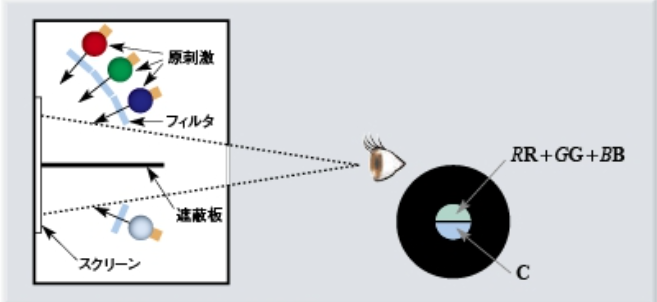
\includegraphics[width=0.5\textwidth]{./figure/022.png}
  \caption{等色実験の原理図}
\end{figure}
\end{frame}

\begin{frame}{CIE-RGB表色系の等色関数}
すべての可視光は,これらの原色の特定の比率で混合することで表現できると考えられている.その混合比を示す関数が等色関数である.
等色関数とは,すべての可視光を表現するために原色の混合比を示す関数である.赤,緑,青のそれぞれの等色関数は \(\bar{r}(\lambda)\), \(\bar{g}(\lambda)\),\(\bar{b}(\lambda)\) とする.ここでの \(\lambda\) はR, G, Bの必要量(刺激値)を表す. ここで,それぞれの等色関数を代入すると,

\begin{equation}\label{eq:cie-rgb}
\textbf{U}(\lambda) = \bar{r}(\lambda)\textbf{R} + \bar{g}(\lambda)\textbf{G} + \bar{b}(\lambda)\textbf{B}
\end{equation}

\(\textbf{U}\)とは,可視光の波長範囲で単位放射量を発行する仮想光のことであり,反射光Cを単一波長光として考え,三刺激値測定したものである.
\begin{figure}
  \centering
  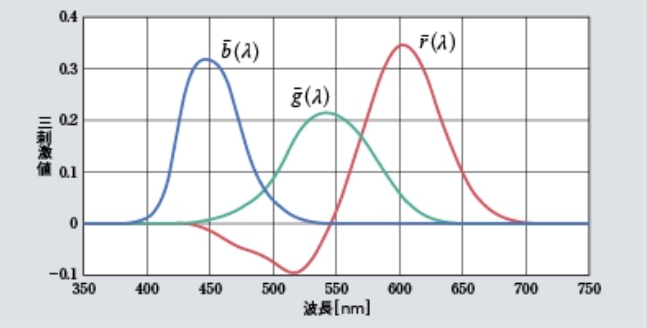
\includegraphics[width=0.5\textwidth]{./figure/023.png}
  \caption{CIE-RGB表色系の等色関数}
  \label{fig:cie-rgb02}
\end{figure}
\end{frame}

\begin{frame}{CIE-RGB表色系の三刺激値}
式\eqref{eq:cie-rgb}より,刺激値の分布を用いることで,反射光のCの分光エネルギー分布
\(L(\lambda)\) から次のように三刺激値R, G, Bを求めることができる.
\begin{equation}
\left\{
\begin{aligned} 
    R = \int_V L(\lambda)\bar{r}(\lambda)d\lambda\\
    G = \int_V L(\lambda)\bar{g}(\lambda)d\lambda\\
    B = \int_V L(\lambda)\bar{b}(\lambda)d\lambda
\end{aligned}
\right.
\end{equation}
ここでの積分範囲 V
は,可視光の波長範囲を表す.したがって,\(\bar{r}(\lambda), \bar{g}(\lambda), \bar{b}(\lambda)\)
が分かれば,任意の分光強度分布を持つ光の色彩を表すことができる.
\end{frame}

\section{CIE-XYZ表色系}
\begin{frame}{CIE-XYZ表色系とは}
CIE-XYZ表色系とは,CIE-RGB表色畏敬の等色関数の問題点であった負の値が存在し,計算のしづらさを解消するために等色関数が非負となるようにCIE-RGB表色系の等色関数から線形変換によって求めた等色関数 \(\bar{x}(\lambda), \bar{y}(\lambda), \bar{z}(\lambda)\)を用いて,三刺激値を求めて表現する.採用された原刺激\(\textbf{X, Y, Z}\) は R,G,Bを用いて表すと,以下のように定義する.
\begin{equation}
\left\{
\begin{pmatrix}
\textbf{X} \\
\textbf{Y} \\
\textbf{Z}
\end{pmatrix}
=
\begin{pmatrix}
0.41844 &  -0.09117 & 0.00092 \\
-0.15866 & 0.25242 & -0.00255 \\
-0.08283 & 0.01570 & 0.17858 \\
\end{pmatrix}
\right. 
\end{equation}
\end{frame}

\begin{frame}{CIE-RGBの原刺激を表し方}
 逆に,CIE-RGB表色系の原刺激 \(\textbf{R, G, B}\) を,三刺激値であるX,Y, Zで表すと
\begin{equation}
\left\{
\begin{pmatrix}
\textbf{R} \\
\textbf{G} \\
\textbf{B}
\end{pmatrix}
= 
\begin{pmatrix}
2.7689 & 1.0000 & 0.0000 \\
1.7517 & 4.5907 & 0.0565 \\
1.1302 & 0.0601 & 5.5943 \\
\end{pmatrix}
\right.
\end{equation}
\end{frame}
\begin{frame}[allowframebreaks,  c]{CIE-XYZ表色系の三刺激値の求め方}
CIE-XYZの表色系では等色実験によって三刺激値を測定することはできないので,CIE-RGBの三刺激値を用いて求める必要がある.
そのための式が式\eqref{eq:xyz-rgb}の座標変換である.
\begin{equation}\label{eq:xyz-rgb}
\begin{pmatrix}
X \\
Y \\
Z
\end{pmatrix}
= 
\begin{pmatrix}
2.7689 & 1.7517 & 1.1302 \\
1.0000 & 4.5907 & 0.0601 \\
0.0000 & 0.0565 & 5.5943 
\end{pmatrix}
\begin{pmatrix}
R \\
G \\
B
\end{pmatrix}
\end{equation}
\newpage

また,等色関数 \(\bar{x}(\lambda), \bar{y}(\lambda), \bar{z}(\lambda)\)
が分かっていれば,三刺激値X, Y, Zを求めることができる. 

\begin{equation}
\left\{
\begin{aligned}
X = \int_V L(\lambda)\bar{x}(\lambda)d\lambda \\
Y = \int_V L(\lambda)\bar{y}(\lambda)d\lambda \\
Z = \int_V L(\lambda)\bar{z}(\lambda)d\lambda
\end{aligned}
\right.
\end{equation}
\begin{figure}
  \centering
  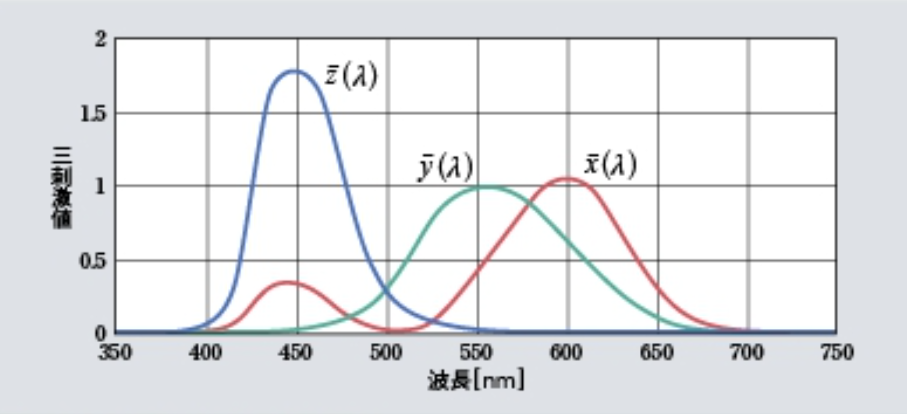
\includegraphics[width=0.5\textwidth]{./figure/029.png}
  \caption{CIE-XYZ表色系の等色関数}
  \label{fig:cie-xyz}
\end{figure}
\end{frame}

\begin{frame}[allowframebreaks]{CIE-XYZ表色系のベクトル表現}
ここで,X, Y, Zを3軸とする直交座標を考えると,任意の色Cは3次元ベクトルで表現できる.
このベクトルは色度座標と呼び,3刺激値を用いて以下で表現できる. 
\begin{equation}
\left\{
\begin{aligned}
    x = \dfrac{X}{X + Y + Z} \\
    y = \dfrac{Y}{X + Y + Z} \\
    z = \dfrac{Z}{X + Y + Z} 
\end{aligned}
\right.
\end{equation}
\begin{block}{}
  \begin{itemize}
    \item \(x\) : 赤の強さを表す成分
    \item \(y\) : 緑の強さを表す成分
    \item \(z\) : 青の強さを表す成分 
  \end{itemize}
\end{block}
\end{frame}

\begin{frame}{xy色度図}
このとき,\(x + y + z = 1\) が成り立つため,3次元座標から2次元座標(x,
y)に変換することができる.これをxy色度図と呼ぶ.
xy色度図の各変数は次のような意味合いを持つ. 
\begin{itemize}
  \item \(x\) : 値が大きいほど赤が強く,値が小さいほど青が強い
  \item \(y\) : 値が大きいほど緑が強く,値が小さいほど青が強い 
\end{itemize}
\begin{figure}
  \centering
  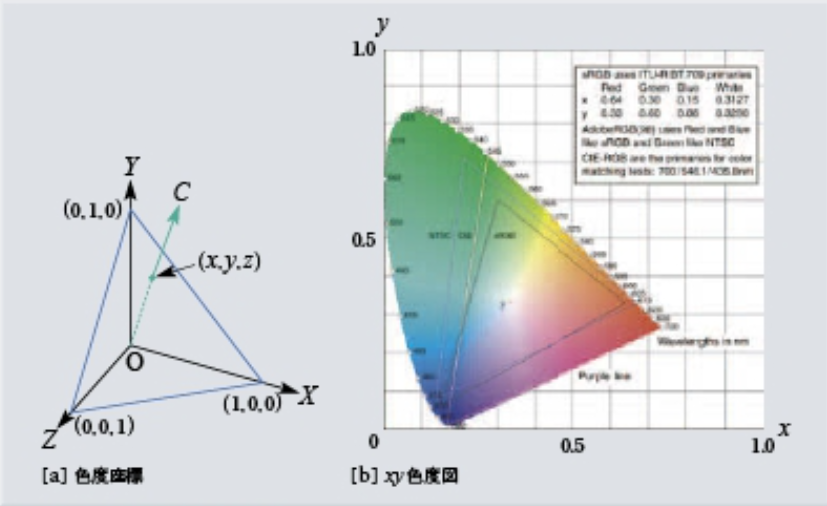
\includegraphics[width=0.5\textwidth]{./figure/028.png}
  \caption{色度座標と色度図}
  \label{fig:xy}
\end{figure}
\end{frame}

\section{CIE-L * a * b * 色空間}
\begin{frame}{CIE-L * a * b * 色空間}
CIE-L * a * b *色空間とは,均等空間の一種であり,異なる2色の色がどの程度似ているのか,どの程度異なっているかを数値化するために用いる.
この色空間は三刺激値(X, Y,
Z)で均等色空間を近似することを目的としており,L*, a*, b*の直交座標系で定義されている. 
\begin{itemize}
  \item L*は明度を示す.0が黒で100に対応している. 
  \item a*は色の赤みと緑の度合いを示す.値が大きいほど赤みが強く,値が小さいほど緑みが強くなる.
  \item b*は色の黄みと青みの度合いを示す.値が大きいほど黄みが強く,値が小さいほどみ青みが強くなる.
\end{itemize}
\begin{figure}
  \centering
  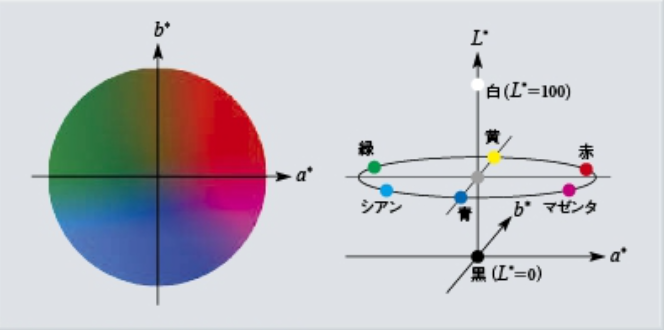
\includegraphics[width=0.5\textwidth]{./figure/024.png}
  \caption{CIE-L * a * b * 色空間}
  \label{fig:cie-lab}
\end{figure}
\end{frame}
\begin{frame}{CIE-L * a * b * 色空間の直交座標系}
\begin{equation}
\left\{
\begin{aligned}
    L* &= 116f\left(\frac{Y}{Y_n}\right)-16 \\
    a* &= 500\left(f\left(\dfrac{X}{X_n}\right) - f\left(\dfrac{Y}{Y_n}\right)\right) \\
    b* &= 200\left(f\left(\dfrac{Y}{Y_n}\right) - f\left(\dfrac{Z}{Z_n}\right)\right) \\
\end{aligned}
\right.
\end{equation}
この関数\(f\)は以下のように定義されている.
\begin{equation}
f(\alpha) =
\left\{
\begin{aligned}
&\alpha^{\frac{1}{3}}, & \alpha > \left(\frac{24}{116}\right)^3 \\
&(\frac{841}{108})\alpha + \frac{16}{116} &\alpha \leqq \left(\frac{24}{116}\right)^3
\end{aligned}
\right.
\end{equation}
\end{frame}

\begin{frame}{CIE-L * a * b * 色空間の色差}
この色空間では,\((L^*_1, a^*_1, b^*_1)\)
と \((L^*_2, a^*_2, b^*_2,)\) の2色間の色差 \(\Delta\)
は,ユークリッド距離として,以下のように計算することができる.
\begin{equation}
\Delta = [(L^*_1- L^*_2)^2 + (a^*_1 - a^*_2)^2 + (b^*_1 - b^*_2)^2]^\frac{1}{2}
\end{equation}
\end{frame}

\section{sRGB色空間}

\begin{frame}{sRGB色空間とは}  
sRGB色空間とは,デバイス独立色の色空間の一種類.
以下の4つの刺激が定義されている.  
\begin{itemize}
\item \(\textbf{R}\) = (0.6400, 0.3300) -
\item \(\textbf{G}\) = (0.3300, 0.6000) 
\item \(\textbf{B}\) = (0.3127, 0.3290) =
\item \(\textbf{W}\) = (0.3127,  0.3290)= (標準光$D_{65}$)
\end{itemize}
\end{frame}

\begin{frame}{sRGB色空間からCIE-XYZ色空間への変換}
sRGB色空間からCIE-XYZの三刺激値に変換する方法を示す.
式\eqref{eq:srgb}は,sRGBの非線形の電気信号 \(E'\) から線形な光の強度 \(E\)
への変換を行う式である.
\begin{equation} \label{eq:srgb}
\begin{aligned}
E'_{sRGB} &= \frac{E'_{8bit}}{255.0} \\
E_{sRGB} &=
\begin{cases}
\dfrac{E'_{sRGB}}{12.92} & E'_{sRGB} \leqq 0.04045 \\
\left(\dfrac{E'_{sRGB} + 0.055}{1.055}\right)^{24} &E'_{sRGB} > 0.4045
\end{cases}
\end{aligned}
\end{equation}
次に,式\eqref{eq:srgb2xyz}では,CIE-XYZ表色系の三刺激値に変換すると 
\begin{equation} \label{eq:srgb2xyz}
\begin{pmatrix}
X \\
Y \\
Z \\
\end{pmatrix}
=
\begin{pmatrix}
0.4124 & 0.3576 & 0.1805 \\
0.2126 & 0.7152 & 0.0722 \\
0.0193 & 0.1192 & 0.9505 
\end{pmatrix}
\begin{pmatrix}
R_{sRGB} \\
G_{sRGB} \\
B_{sRGB}
\end{pmatrix}
\end{equation}
\end{frame}

\begin{frame}{sRGB色空間からCIE-XYZ色空間への逆変換}
式\eqref{eq:xyz2srgb}は,CIE-XYZ表色系の三刺激値からsRGB色空間に変換する方法を以下に示す.
\begin{equation}\label{eq:xyz2srgb}
\begin{pmatrix}
R_{\text{sRGB}} \\
G_{\text{sRGB}} \\
B_{\text{sRGB}}
\end{pmatrix}
=
\begin{pmatrix}
3.2406 & -1.5372 & -0.4989 \\
-0.9689 & 1.8578 & 0.0415 \\
0.0557 & -0.2040 & 1.0570
\end{pmatrix}
\begin{pmatrix}
X \\
Y \\
Z
\end{pmatrix}
\end{equation}

\(\gamma = 2.2\) に対するガンマ補正を行い,0から255までの8ビット
線形なsRGB値 \(E_{sRGB}\)から非線形な8bit値\(E'_{8bit}\)への変換を式\eqref{eq:gamma}行う.
\begin{equation}\label{eq:gamma}
\begin{aligned}
E'_{sRGB} &=
\begin{cases}
12.92 E_{sRGB} & E_{sRGB} \leqq 0.0031308 \\
1.055 E_{sRGB}^{\frac{1}{2.4}} - 0.055 & E_{sRGB} > 0.0031308 \\
\end{cases} \\
E'_{8bit} &=255.0E'_{sRGB}
\end{aligned}
\end{equation}
\end{frame}

\section{輝度信号と色差信号}
\begin{frame}{輝度信号と色差信号}
人間の目は,色の変化よりも明るさの変化に対して敏感である.そのため,輝度成分はそのまま保持し,色の情報については情報を減らしたりしても,視覚的な劣化を知覚しづらいという特性を持つ.テレビ放送でもRGB値を輝度成分と色差成分に変換している.
これを利用した変換の1つがYUV変換である. 
\begin{itemize}
  \item Yは明るさを表す輝度信号 
  \item Uは青みと輝度成分の差を表す.値が大きいと青みが強く,小さいほど黄色みが強くなる
  \item Vは赤色と輝度成分の差を表す.値が大きいと赤みが強く,小さいほど緑みが強くなる
\end{itemize}
式\eqref{eq:yuv}は,RGB値からYUV変換を行う式である.
\begin{equation} \label{eq:yuv}
\begin{cases}
Y &= 0.299R' + 0.587G' + 0.114B' \\
U &= 0.492(B' - Y) = 0.147R' - 0.289G' + 0.436B' \\
V &= 0.877(R' - Y) = 0.615R' - 0.515G' - 0.100B' \\
\end{cases}
\end{equation}
\end{frame}

\begin{frame}[allowframebreaks]{YCbCr変換}
この色空間は,基本となる赤,緑,青の光の色合いと基準となる白の色合いをxy色度変換という方法で定義している.また,これらの原色を用いて色を表すRGB値は\(\gamma = 2.2\)
という特性でガンマ補正されており,0 \textasciitilde 1までの値をとる.
\begin{equation}
\begin{aligned}
    \textbf{R} &= (0.6400, 0.3300) \\
    \textbf{G} &= (0.2900, 0.6000) \\
    \textbf{B} &= (0.1500, 0.0600) \\
    \textbf{W} &= (0.3127, 03290) (\text{標準光}D_{65})
\end{aligned}
\end{equation}
YCbCr変換は,YUV変換と似ているが色差信号の信号が異なる.
YUV変換では負の値を含むことがあるため,デジタル環境での扱いやすさを考慮して,負の値を含まないようにオフセットしている.
\newpage

静止画像の代表的な圧縮フォーマットであるJPEGは以下のような方法で変換している.
この式は,RGB値からYCbCr変換を行っている.
\begin{equation}
\begin{cases}
Y &= 0.299R' + 0.587G' + 0.114B' \\
C_b &= 0.564(B' - Y) = -0.169R' - 0.331G' + 0.500B' \\
C_r &= 0.713(R' - Y) = 0.500R' - 0.419G' -0.081B'
\end{cases}
\end{equation}
 sRGB値からのYCbCr変換は以下のような式で求めることができる.
\begin{equation}
\begin{cases}
Y &= 02126R' + 07152G' + 0.0722B' \\
G &= 0.5389(B' - Y) = -0.1146R' - 0.3854G' + 0.5000B' \\
B &= 0.6350(R' - Y) = 0.5000R' - 0.4542G' - 0.0458B'
\end{cases}
\end{equation}
\end{frame}

\section{HSI変換と逆変換}
\begin{frame}{HSI変換とは}
HSI変換とは,色相・彩度・明度を座標軸とする変換のことである.この変換を用いることでRGB値では色の濃さと画像の明るさが連動してしまうという問題点があったが,HSI変換を用いることで画像の明るさと彩度を別で変更させたい場合はHSI変換を用いることで解決する.
\end{frame}

\begin{frame}[allowframebreaks]{6角錐モデル}
このモデルのHSI変換は以下の通りとなっている.

\begin{equation}
\begin{aligned}
I_{max} &= max\{R, G, B\}, I_{min} = min\{R, G, B\} \\
I &= I_{max} \\
S &= (I_{max} - I_{min}) / I_{max} \\
H &= 
\begin{cases}
\dfrac{G - B}{I_{max} - I_{min}}\dfrac{\pi}{3} & (I_{max} = R) \\[3mm]
\dfrac{B - R}{I_{max} - I_{min}}\dfrac{\pi}{3} + \dfrac{2}{3}\pi & (I_{max} = G) \\[3mm]
\dfrac{R - G}{I_{max} - I_{min}}\dfrac{\pi}{3} + \dfrac{4}{3}\pi & (I_{max} = B)
\end{cases}
\end{aligned}
\end{equation}
\newpage
\begin{figure}[b]
  \centering
  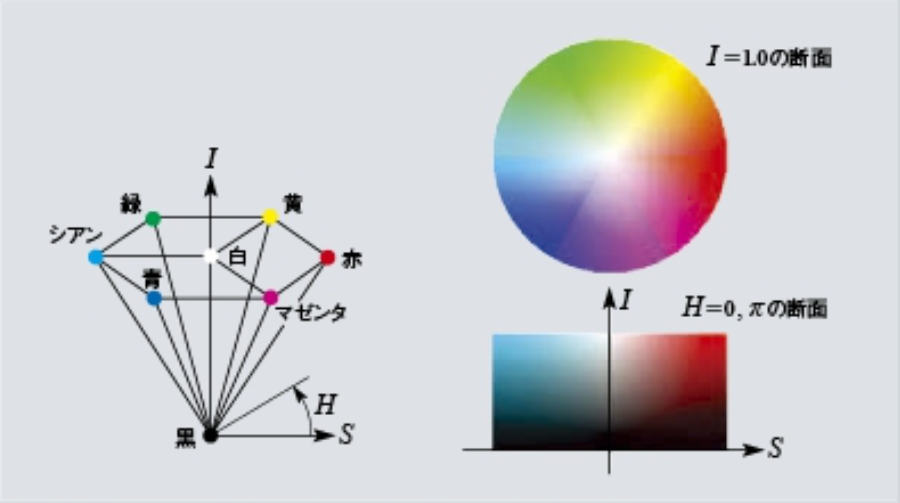
\includegraphics[width=0.5\textwidth]{./figure/026.png}
  \caption{HSI変換の6角錐モデル}
  \label{fig:hsi}
\end{figure}

\newpage

これの逆変換について以下のようになる.
\begin{equation}
 (R,G,B) =
\begin{cases}
(I, T, P) & (h = 0) \\
(Q, I, P) & (h = 1) \\
(P, I, T) & (h = 2) \\
(P, Q, T) & (h = 3) \\
(T, P, I) & (h = 4) \\
(I, P, Q) & (h = 5) \\
\end{cases}
\end{equation}
各値は以下のように表現することができる
\begin{equation}
\begin{aligned}
h &= floor(\dfrac{3}{\pi}H) \\
P &= I(1 - S) \\
Q &= I(1 - S(\dfrac{3}{\pi}H - h)) \\
T &= I(1  - S(1 - \dfrac{3}{\pi} H + h)) \\
\end{aligned}
\begin{aligned}
&H = 2\pi = 0 \\
&0 \leqq R, G, B, S, I \leqq 1 \\
&0 \leqq H < 2\pi
\end{aligned}
\end{equation}
\end{frame}


\begin{frame}[allowframebreaks]{双6角錐モデル}
6角錐モデルをより精密にしたもの.デザイン分野で利用されるオズワルド表色系に近い.

\begin{equation}
\begin{aligned}
I_{max} &= max\{R, G, B\}, ~~ I_{min} = min\{R, G, B\} \\
I &= I_{max} + I+{min} / 2 \\
S &= 
\begin{cases}
\dfrac{I_{max} - I_{min}}{I_{max} + I_{min}} &(I \leqq 0.5)\\[3mm] 
\dfrac{I_{max} - I_{min}}{2 - (I_{max} + I_{min})} &(I >0.5)\\
\end{cases}
\\
H &= 
\begin{cases}
\dfrac{G - B}{I_{max} - I_{min}}\dfrac{\pi}{3} & (I_{max} = R) \\[3mm]
\dfrac{B - R}{I_{max} - I_{min}}\dfrac{\pi}{3} + \dfrac{2}{3}\pi & (I_{max} = G) \\[3mm]
\dfrac{R - G}{I_{max} - I_{min}}\dfrac{\pi}{3} + \dfrac{4}{3}\pi & (I_{max} = B)
\end{cases}
\end{aligned}
\end{equation}

\newpage

\begin{figure}[b]
  \centering
  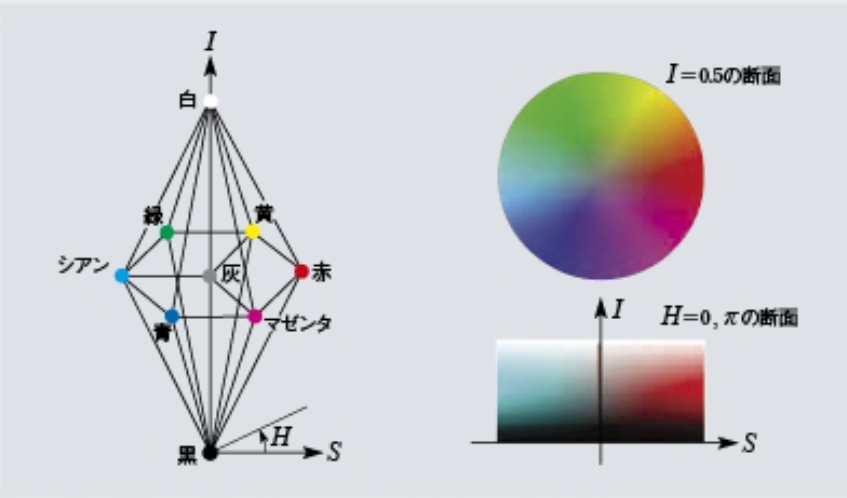
\includegraphics[width=0.5\textwidth]{./figure/027.png}
  \caption{HSI変換の双6角錐モデル}
  \label{fig:hsi2}
\end{figure}


逆変換は,以下のようになる

\begin{equation}
\begin{aligned}
R &= X & (h = H + \frac{2}{3}\pi) \\
G &= X & (h = H) \\
B &= X & (h = H - \frac{2}{3}\pi)
\end{aligned}
\end{equation}


\newpage
X は h に応じて以下のように求めることができる. 

\begin{equation}
\begin{aligned}
h' &=
\begin{cases}
    h \\
    h + 2 \pi & (h < 0) \\ 
    h - 2 \pi & (h > 2\pi) \\
\end{cases}
\\
M_2 &= 
\begin{cases}
    I(1 + S) & (I \leqq 0.5) \\
    I + S - IS & (I > 0.5) \\
\end{cases}
\\
M_1 &= 2I - M_2 \\
X &= 
\begin{cases}
M_1 + \left(M_2 - M_1\right) \frac{3}{\pi}h' & \left(h' < \dfrac{3}{\pi}\right) \\
M_2 & \left(\dfrac{3}{\pi} \leqq h' < \pi\right) \\
M_1 + \left(M_2 - M_1\right)\left(4 - \dfrac{3}{\pi}h'\right) & \left(\pi \leqq h' < \dfrac{4}{3}\pi\right) \\
M_1 & \left(\dfrac{4}{3}\pi \leqq h' \leqq 2\pi\right)
\end{cases}
\end{aligned}
\end{equation}

\end{frame}

\end{document}
